% Model architecture of the TriField surrogate (rendered to assets/architecture.png
% by assets/build_architecture.sh; needs pdflatex + pdftocairo).
\documentclass[tikz,border=6pt]{standalone}
\usepackage{amsmath,amssymb}
\usepackage[T1]{fontenc}
\usepackage{helvet}
\renewcommand{\familydefault}{\sfdefault}
\usetikzlibrary{positioning,arrows.meta,calc,fit,backgrounds,shapes.misc}

\definecolor{cData}{HTML}{E8F1FB}
\definecolor{cDataL}{HTML}{3A6FB0}
\definecolor{cMLP}{HTML}{E6F4EA}
\definecolor{cMLPL}{HTML}{2E7D32}
\definecolor{cGAT}{HTML}{FFF1E0}
\definecolor{cGATL}{HTML}{D9730D}
\definecolor{cOut}{HTML}{F3E8FB}
\definecolor{cOutL}{HTML}{7B3FA0}
\definecolor{cLoss}{HTML}{FDECEC}
\definecolor{cLossL}{HTML}{C62828}
\definecolor{cInk}{HTML}{263238}

\begin{document}
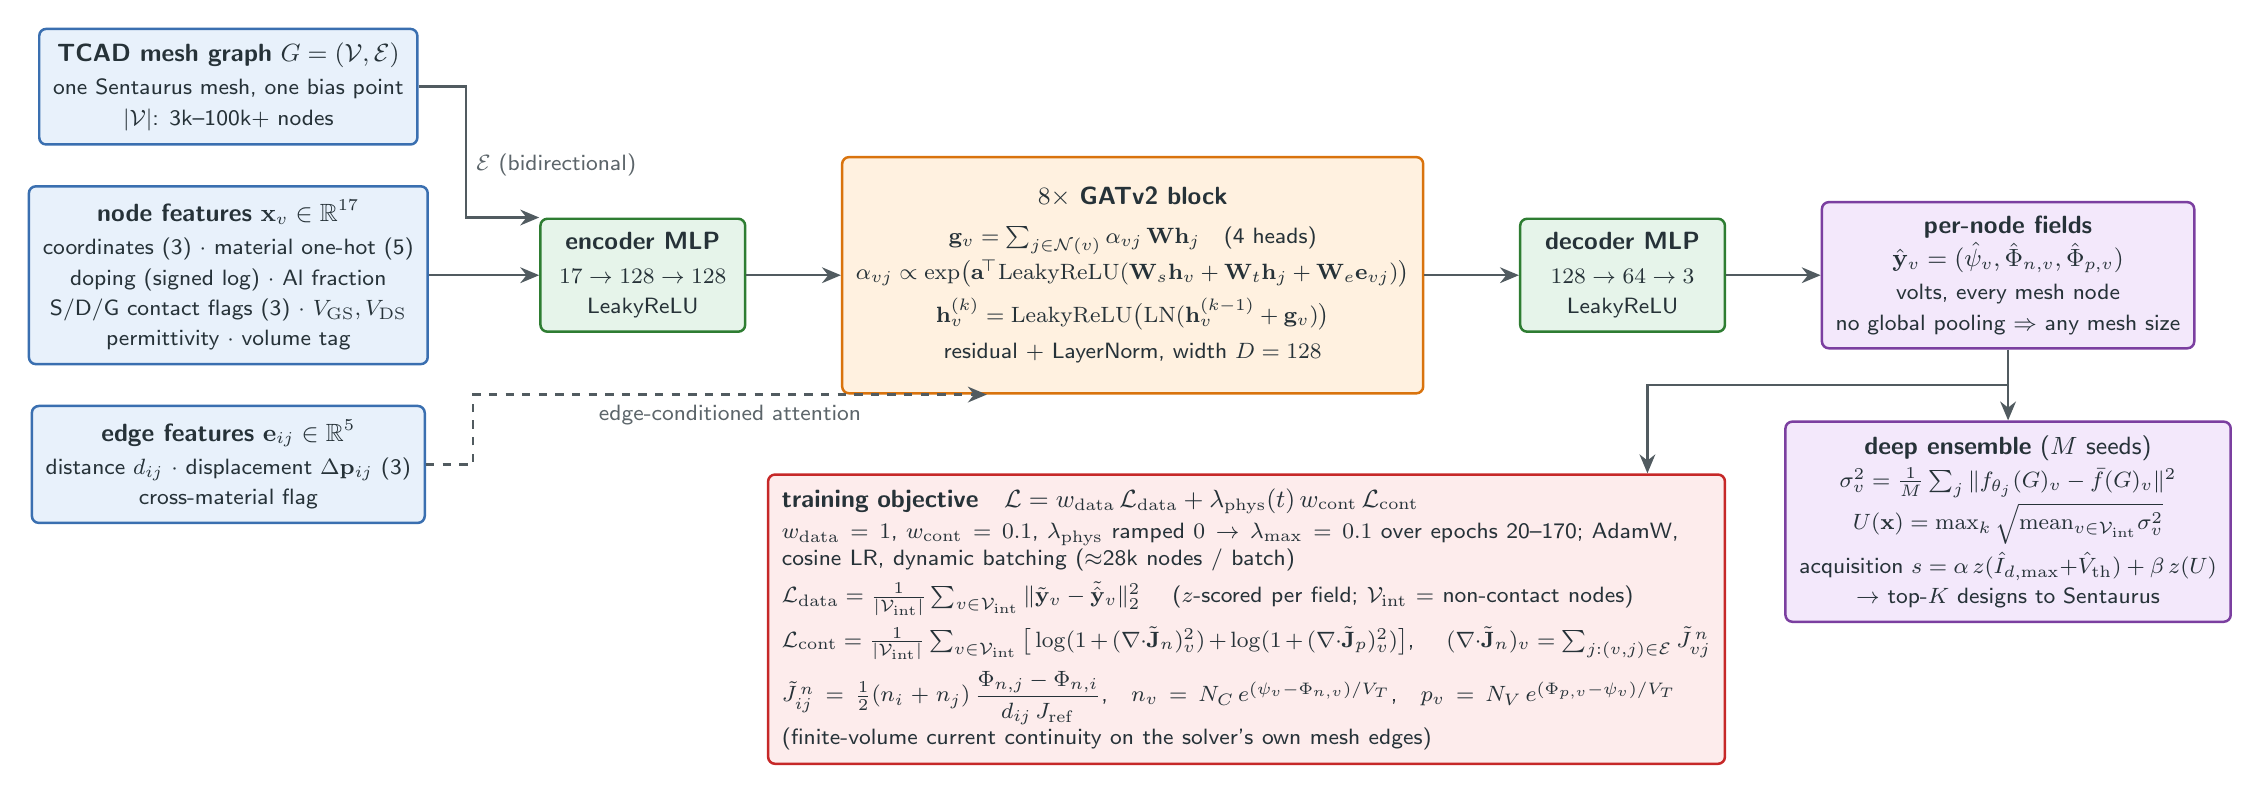
\begin{tikzpicture}[
    font=\small, text=cInk, >={Stealth[length=2.4mm,width=2mm]},
    box/.style={draw, line width=0.9pt, rounded corners=2.5pt, align=center,
                inner sep=5pt, minimum height=11mm},
    data/.style={box, fill=cData, draw=cDataL},
    mlp/.style={box, fill=cMLP, draw=cMLPL},
    gat/.style={box, fill=cGAT, draw=cGATL},
    outp/.style={box, fill=cOut, draw=cOutL},
    loss/.style={box, fill=cLoss, draw=cLossL},
    arr/.style={->, line width=0.9pt, color=cInk!80},
    lbl/.style={font=\footnotesize, text=cInk!75, align=center},
]

% ---------------- inputs ----------------
\node[data, minimum width=36mm] (mesh) {\textbf{TCAD mesh graph} $G=(\mathcal V,\mathcal E)$\\[1pt]
    \footnotesize one Sentaurus mesh, one bias point\\
    \footnotesize $|\mathcal V|$: 3k--100k+ nodes};

\node[data, below=5mm of mesh, minimum width=36mm] (xv) {\textbf{node features} $\mathbf x_v\in\mathbb R^{17}$\\[1pt]
    \footnotesize coordinates (3) $\cdot$ material one-hot (5)\\
    \footnotesize doping (signed log) $\cdot$ Al fraction\\
    \footnotesize S/D/G contact flags (3) $\cdot$ $V_{\mathrm{GS}},V_{\mathrm{DS}}$\\
    \footnotesize permittivity $\cdot$ volume tag};

\node[data, below=5mm of xv, minimum width=36mm] (eij) {\textbf{edge features} $\mathbf e_{ij}\in\mathbb R^{5}$\\[1pt]
    \footnotesize distance $d_{ij}$ $\cdot$ displacement $\Delta\mathbf p_{ij}$ (3)\\
    \footnotesize cross-material flag};

% ---------------- network ----------------
\node[mlp, right=14mm of xv, minimum width=26mm] (enc) {\textbf{encoder MLP}\\[1pt] \footnotesize $17\to128\to128$\\ \footnotesize LeakyReLU};

\node[gat, right=12mm of enc, minimum width=46mm, minimum height=30mm] (gat) {
    \textbf{$8\times$ GATv2 block}\\[3pt]
    \footnotesize $\mathbf g_v=\sum_{j\in\mathcal N(v)}\alpha_{vj}\,\mathbf W\mathbf h_j$\quad (4 heads)\\[2pt]
    \footnotesize $\alpha_{vj}\propto\exp\!\big(\mathbf a^{\!\top}\mathrm{LeakyReLU}(\mathbf W_s\mathbf h_v+\mathbf W_t\mathbf h_j+\mathbf W_e\mathbf e_{vj})\big)$\\[3pt]
    \footnotesize $\mathbf h_v^{(k)}=\mathrm{LeakyReLU}\big(\mathrm{LN}(\mathbf h_v^{(k-1)}+\mathbf g_v)\big)$\\[2pt]
    \footnotesize residual + LayerNorm, width $D=128$};

\node[mlp, right=12mm of gat, minimum width=26mm] (dec) {\textbf{decoder MLP}\\[1pt] \footnotesize $128\to64\to3$\\ \footnotesize LeakyReLU};

\node[outp, right=12mm of dec, minimum width=30mm] (y) {\textbf{per-node fields}\\[1pt]
    $\hat{\mathbf y}_v=(\hat\psi_v,\hat\Phi_{n,v},\hat\Phi_{p,v})$\\[1pt]
    \footnotesize volts, every mesh node\\ \footnotesize no global pooling $\Rightarrow$ any mesh size};

% edge features feed the attention
\draw[arr, dashed] (eij.east) -- ++(6mm,0) |- ($(gat.south west)!0.5!(gat.south)$) node[pos=0.75, below, lbl] {edge-conditioned attention};

\draw[arr] (xv) -- (enc);
\draw[arr] (enc) -- (gat);
\draw[arr] (gat) -- (dec);
\draw[arr] (dec) -- (y);
\draw[arr] (mesh.east) -- ++(6mm,0) |- (enc.north west) node[pos=0.3, right, lbl] {$\mathcal E$ (bidirectional)};

% ---------------- training objective ----------------
\node[loss, anchor=north east, text width=118mm, align=left]
    at ($(dec.east |- gat.south)+(0,-10mm)$) (loss) {
    \textbf{training objective}\quad
    $\mathcal L=w_{\mathrm{data}}\,\mathcal L_{\mathrm{data}}+\lambda_{\mathrm{phys}}(t)\,w_{\mathrm{cont}}\,\mathcal L_{\mathrm{cont}}$\\[2pt]
    \footnotesize $w_{\mathrm{data}}=1$,\ $w_{\mathrm{cont}}=0.1$,\ $\lambda_{\mathrm{phys}}$ ramped $0\to\lambda_{\max}=0.1$ over epochs 20--170;\ AdamW, cosine LR, dynamic batching ($\approx$28k nodes / batch)\\[3pt]
    \footnotesize $\mathcal L_{\mathrm{data}}=\frac{1}{|\mathcal V_{\mathrm{int}}|}\sum_{v\in\mathcal V_{\mathrm{int}}}\|\tilde{\mathbf y}_v-\tilde{\hat{\mathbf y}}_v\|_2^2$
    \quad ($z$-scored per field; $\mathcal V_{\mathrm{int}}$ = non-contact nodes)\\[3pt]
    \footnotesize $\mathcal L_{\mathrm{cont}}=\frac{1}{|\mathcal V_{\mathrm{int}}|}\sum_{v\in\mathcal V_{\mathrm{int}}}\big[\log(1+(\nabla\!\cdot\!\tilde{\mathbf J}_n)_v^2)+\log(1+(\nabla\!\cdot\!\tilde{\mathbf J}_p)_v^2)\big]$,
    \quad $(\nabla\!\cdot\!\tilde{\mathbf J}_n)_v=\sum_{j:(v,j)\in\mathcal E}\tilde J^{\,n}_{vj}$\\[3pt]
    \footnotesize $\tilde J^{\,n}_{ij}=\tfrac{1}{2}(n_i+n_j)\,\dfrac{\Phi_{n,j}-\Phi_{n,i}}{d_{ij}\,J_{\mathrm{ref}}}$,\quad
    $n_v=N_C\,e^{(\psi_v-\Phi_{n,v})/V_T}$,\quad $p_v=N_V\,e^{(\Phi_{p,v}-\psi_v)/V_T}$
    \quad (finite-volume current continuity on the solver's own mesh edges)};



% ---------------- ensemble / active learning ----------------
\node[outp, below=9mm of y, minimum width=34mm, align=center] (al) {
    \textbf{deep ensemble} ($M$ seeds)\\[1pt]
    \footnotesize $\sigma_v^2=\frac1M\sum_j\|f_{\theta_j}(G)_v-\bar f(G)_v\|^2$\\[1pt]
    \footnotesize $U(\mathbf x)=\max_k\sqrt{\mathrm{mean}_{v\in\mathcal V_{\mathrm{int}}}\sigma_v^2}$\\[2pt]
    \footnotesize acquisition $s=\alpha\,z(\hat I_{d,\max}{+}\hat V_{\mathrm{th}})+\beta\,z(U)$\\
    \footnotesize $\to$ top-$K$ designs to Sentaurus};
\draw[arr] (y.south) -- (al.north);
\draw[arr] ($(y.south)!0.5!(al.north)$) -| ($(loss.north east)+(-10mm,0)$);

\end{tikzpicture}
\end{document}
